\documentclass[11pt,a4paper]{article}
\usepackage[margin=2.5cm]{geometry}
\usepackage{graphicx}
\usepackage{float}
\usepackage{amsmath}

\title{Report 5: Gaussian Blur}
\author{Le Nguyen Minh Quang (2540093)}
\date{\today}

\begin{document}
\maketitle

\section{Goal}
In this labwork I changed my grayscale kernel from labwork 4 into a 7x7
Gaussian blur. I wrote two versions, one without shared memory and one
with shared memory. Then I tested different block sizes. I ran
everything on Google Colab with a Tesla T4 GPU. My image is 1200x750
pixels.

\section{How I implemented it}
I used the 7x7 filter from the slides. The sum of all values is 1003.
\[
\begin{bmatrix}
0 & 0 & 1 & 2 & 1 & 0 & 0 \\
0 & 3 & 13 & 22 & 13 & 3 & 0 \\
1 & 13 & 59 & 97 & 59 & 13 & 1 \\
2 & 22 & 97 & 159 & 97 & 22 & 2 \\
1 & 13 & 59 & 97 & 59 & 13 & 1 \\
0 & 3 & 13 & 22 & 13 & 3 & 0 \\
0 & 0 & 1 & 2 & 1 & 0 & 0
\end{bmatrix}
\]
For each pixel and each colour, I multiply the 49 neighbours by the
filter and add them together. Then I divide by the sum of the weights.
If a neighbour is outside the image, I skip it.

On the GPU I use the same 2D grid as in labwork 4, so one thread
computes one pixel.

\subsection{Without shared memory}
Here every thread reads the filter from global memory.
\begin{verbatim}
@cuda.jit
def blur(src, dst, filt):
    tidx = cuda.threadIdx.x + cuda.blockIdx.x * cuda.blockDim.x
    tidy = cuda.threadIdx.y + cuda.blockIdx.y * cuda.blockDim.y
    if tidy < src.shape[0] and tidx < src.shape[1]:
        for c in range(3):
            total = 0
            weightSum = 0
            for i in range(7):
                for j in range(7):
                    ny = tidy + i - 3
                    nx = tidx + j - 3
                    if ny >= 0 and ny < src.shape[0] and
                       nx >= 0 and nx < src.shape[1]:
                        total += filt[i, j] * src[ny, nx, c]
                        weightSum += filt[i, j]
            dst[tidy, tidx, c] = np.uint8(total / weightSum)
\end{verbatim}

\subsection{With shared memory}
Like in the slides, each block first copies the filter into shared
memory. Then all threads wait until the filter is ready, using
cuda.syncthreads(). After that the code is the same, but it reads the
filter from sFilter.
\begin{verbatim}
sFilter = cuda.shared.array((7, 7), numba.int32)
if cuda.threadIdx.x < 7 and cuda.threadIdx.y < 7:
    tx = cuda.threadIdx.x
    ty = cuda.threadIdx.y
    sFilter[ty, tx] = filt[ty, tx]
cuda.syncthreads()
\end{verbatim}
Only the first 7x7 threads copy the filter, so the block must have at
least 7x7 threads. That is why my smallest block is 8x8.

\section{Results}
The CPU took 192.67 seconds. Both GPU versions give exactly the same
image as the CPU.

\begin{figure}[H]
  \centering
  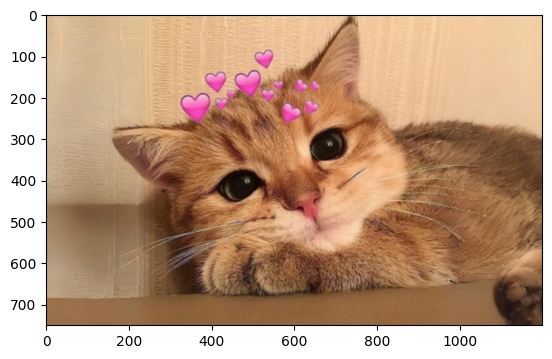
\includegraphics[width=0.6\textwidth]{blur_gpu.png}
  \caption{My image after the Gaussian blur.}
\end{figure}

I ran each kernel 50 times and took the average time.
Speedup is CPU time divided by GPU time.

\begin{center}
\begin{tabular}{|c|c|c|c|c|}
\hline
Block & Time without shared & Speedup & Time with shared & Speedup \\ \hline
8x8   & 1.94 ms & 99254  & 1.83 ms & 105408 \\ \hline
12x12 & 1.91 ms & 100926 & 1.00 ms & 192699 \\ \hline
16x16 & 0.93 ms & 206311 & 0.96 ms & 199727 \\ \hline
24x24 & 1.16 ms & 166379 & 1.03 ms & 187874 \\ \hline
32x32 & 0.90 ms & 215022 & 0.92 ms & 210442 \\ \hline
\end{tabular}
\end{center}

\begin{figure}[H]
  \centering
  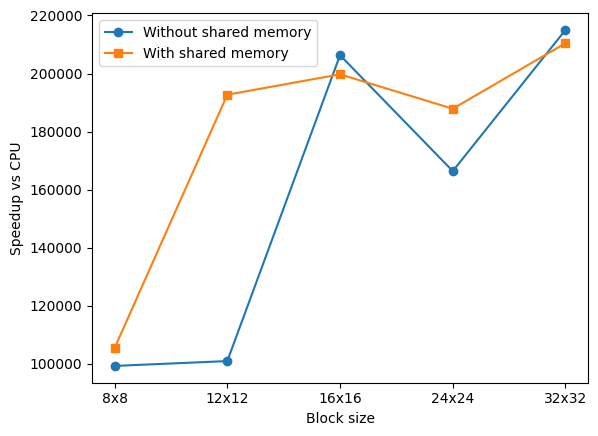
\includegraphics[width=0.7\textwidth]{blocksize_vs_speedup.png}
  \caption{Block size vs speedup.}
\end{figure}

\section{Discussion}
The GPU is much faster than the CPU. The blur needs 49 neighbours for
every pixel, so the CPU needs more than 3 minutes, but the GPU only
needs about 1 ms.

The 8x8 block is the slowest. The 16x16 and 32x32 blocks are the
fastest.

Shared memory does not help much. With 16x16 and 32x32 the two
versions have almost the same time. I think this is because the filter
is very small (only 49 numbers), so the GPU already keeps it in cache.
Most of the time is spent reading the image pixels, and both versions
still read them from global memory. The big difference at 12x12 is
probably just noise in the measurement.

\section{Conclusion}
My Gaussian blur works on the GPU and gives the same result as the CPU.
It is about 200000 times faster. The best block size is 32x32 or
16x16. Putting only the filter in shared memory does not change the
speed much.

\end{document}
